\documentclass{article}
\usepackage{graphicx}
\usepackage[letterpaper, total={6.5in, 9in}]{geometry}
\usepackage{listings}

\usepackage{xcolor}

\definecolor{codegreen}{rgb}{0,0.6,0}
\definecolor{codegray}{rgb}{0.5,0.5,0.5}
\definecolor{codepurple}{rgb}{0.58,0,0.82}
\definecolor{backcolour}{rgb}{0.95,0.95,0.92}

\lstdefinestyle{mystyle}{
    backgroundcolor=\color{backcolour},   
    commentstyle=\color{codegreen},
    keywordstyle=\color{magenta},
    numberstyle=\tiny\color{codegray},
    stringstyle=\color{codepurple},
    basicstyle=\ttfamily\footnotesize,
    breakatwhitespace=false,         
    breaklines=true,                 
    captionpos=b,                    
    keepspaces=true,                 
    numbers=left,                    
    numbersep=5pt,                  
    showspaces=false,                
    showstringspaces=false,
    showtabs=false,                  
    tabsize=4
}

\lstset{style=mystyle}

\title{Project 2: Digital Inputs and Interrupts Solution}

\author{Braidan Duffy\thanks{B.S. Ocean Engineering 2021\\M.S. Ocean Engineering 2023}}

\date{May 25, 2022}

\begin{document}

\maketitle

\section*{Overview}
Students will be considered to have completed the project when they demonstrate the following tasks:

\begin{enumerate}
    \item integrated three buttons inputs and three LED outputs with their Arduino
        \subitem one button must have an unfiltered input
        \subitem one button must have a software-regulated input
        \subitem one button must have a hardware RC low-pass filter circuit
    \item implemented three appropriate Interrupt Service Routines (ISRs) into their program
        \subitem each ISR must increment a counter for each button pressed
        \subitem each ISR must send the counter through the Serial port with an appropriate label
    \item showed that the LED state switches and the counter is printed to the serial monitor with every button press   
\end{enumerate}

\section*{Grading}
\begin{tabular}{ | p{1in} | p{1.75in} | p{1.75in} | p{1.75in} | }
    \hline
    \textbf{Category} & \textbf{No Credit} & \textbf{Half Credit} & \textbf{Full Credit} \\

    \hline
    Efficacy (60 pts) & 
    Student did not demonstrate their working project & 
    student demonstrated a working project, but it did not meet all of the requirements specified in the project handout & 
    student demonstrated a feature-complete project that accomplished all of the goals specified in the project handout \\
    \hline
    Printout of Serial monitor (20 pts) & 
    Student did not provide a printout of the Serial monitor &
    Student provided a printout, but it was not appropriately labeled or incoherent&
    Student provided an acceptable printout \\
    \hline
    Schematic neatness (10 pts) & 
    Student did not provide a schematic, or it is illegible &
    Student provided a schematic, but it is difficult to read or understand &
    Student provided a schematic that is easy to read and understand \\
    \hline
    Code neatness (10 pts) & 
    Student did not provide code, or it is difficult to read and follow &
    Student provided code, but it is difficult to read, variable names are nonsensical, functions are not documented or commented, code structure is not helpful &
    Student provided well-documented, easy to read and follow code pursuant to best coding practices and/or C++ standards \\
    \hline
    Mystery extra credit &
    Student did not request extra credit or reach the necessary thresholds & 
    &
    Student successfully implemented a button hold feature \\

    \hline
\end{tabular}

    \subsection*{Extra Credit}
    Students will be granted extra credit if they demonstrated that they change the LED state for the appropriate button after it being held for a determined time. 
    \textbf{Note:} the respective counter should still increment as normal, when the button is pressed.

\section*{Guide}
    \subsection*{Wiring the Breadboard}
    Students should have three buttons and three LEDs on their breadboard connected to the Arduino's GPIO pins.
    The GND pin of the Arduino should be connected to the negative (blue) rail of the breadboard.
    Each LED should have a current-limiting resistor in series with the anode (long wire) and the Arduino output pin with the cathode (short pin) connected to  the negative rail.
    Two buttons should have a 10k-ohm pulldown resistor on one contact end to the negative rail and the other contact end connected directly to an interrupt-capable input pin.
    The third button should have an RC circuit in series with the Arduino input wire as shown in Figure \ref{fig:p2_digital_inputs_bb}. 

    \begin{figure*}
        \centering
        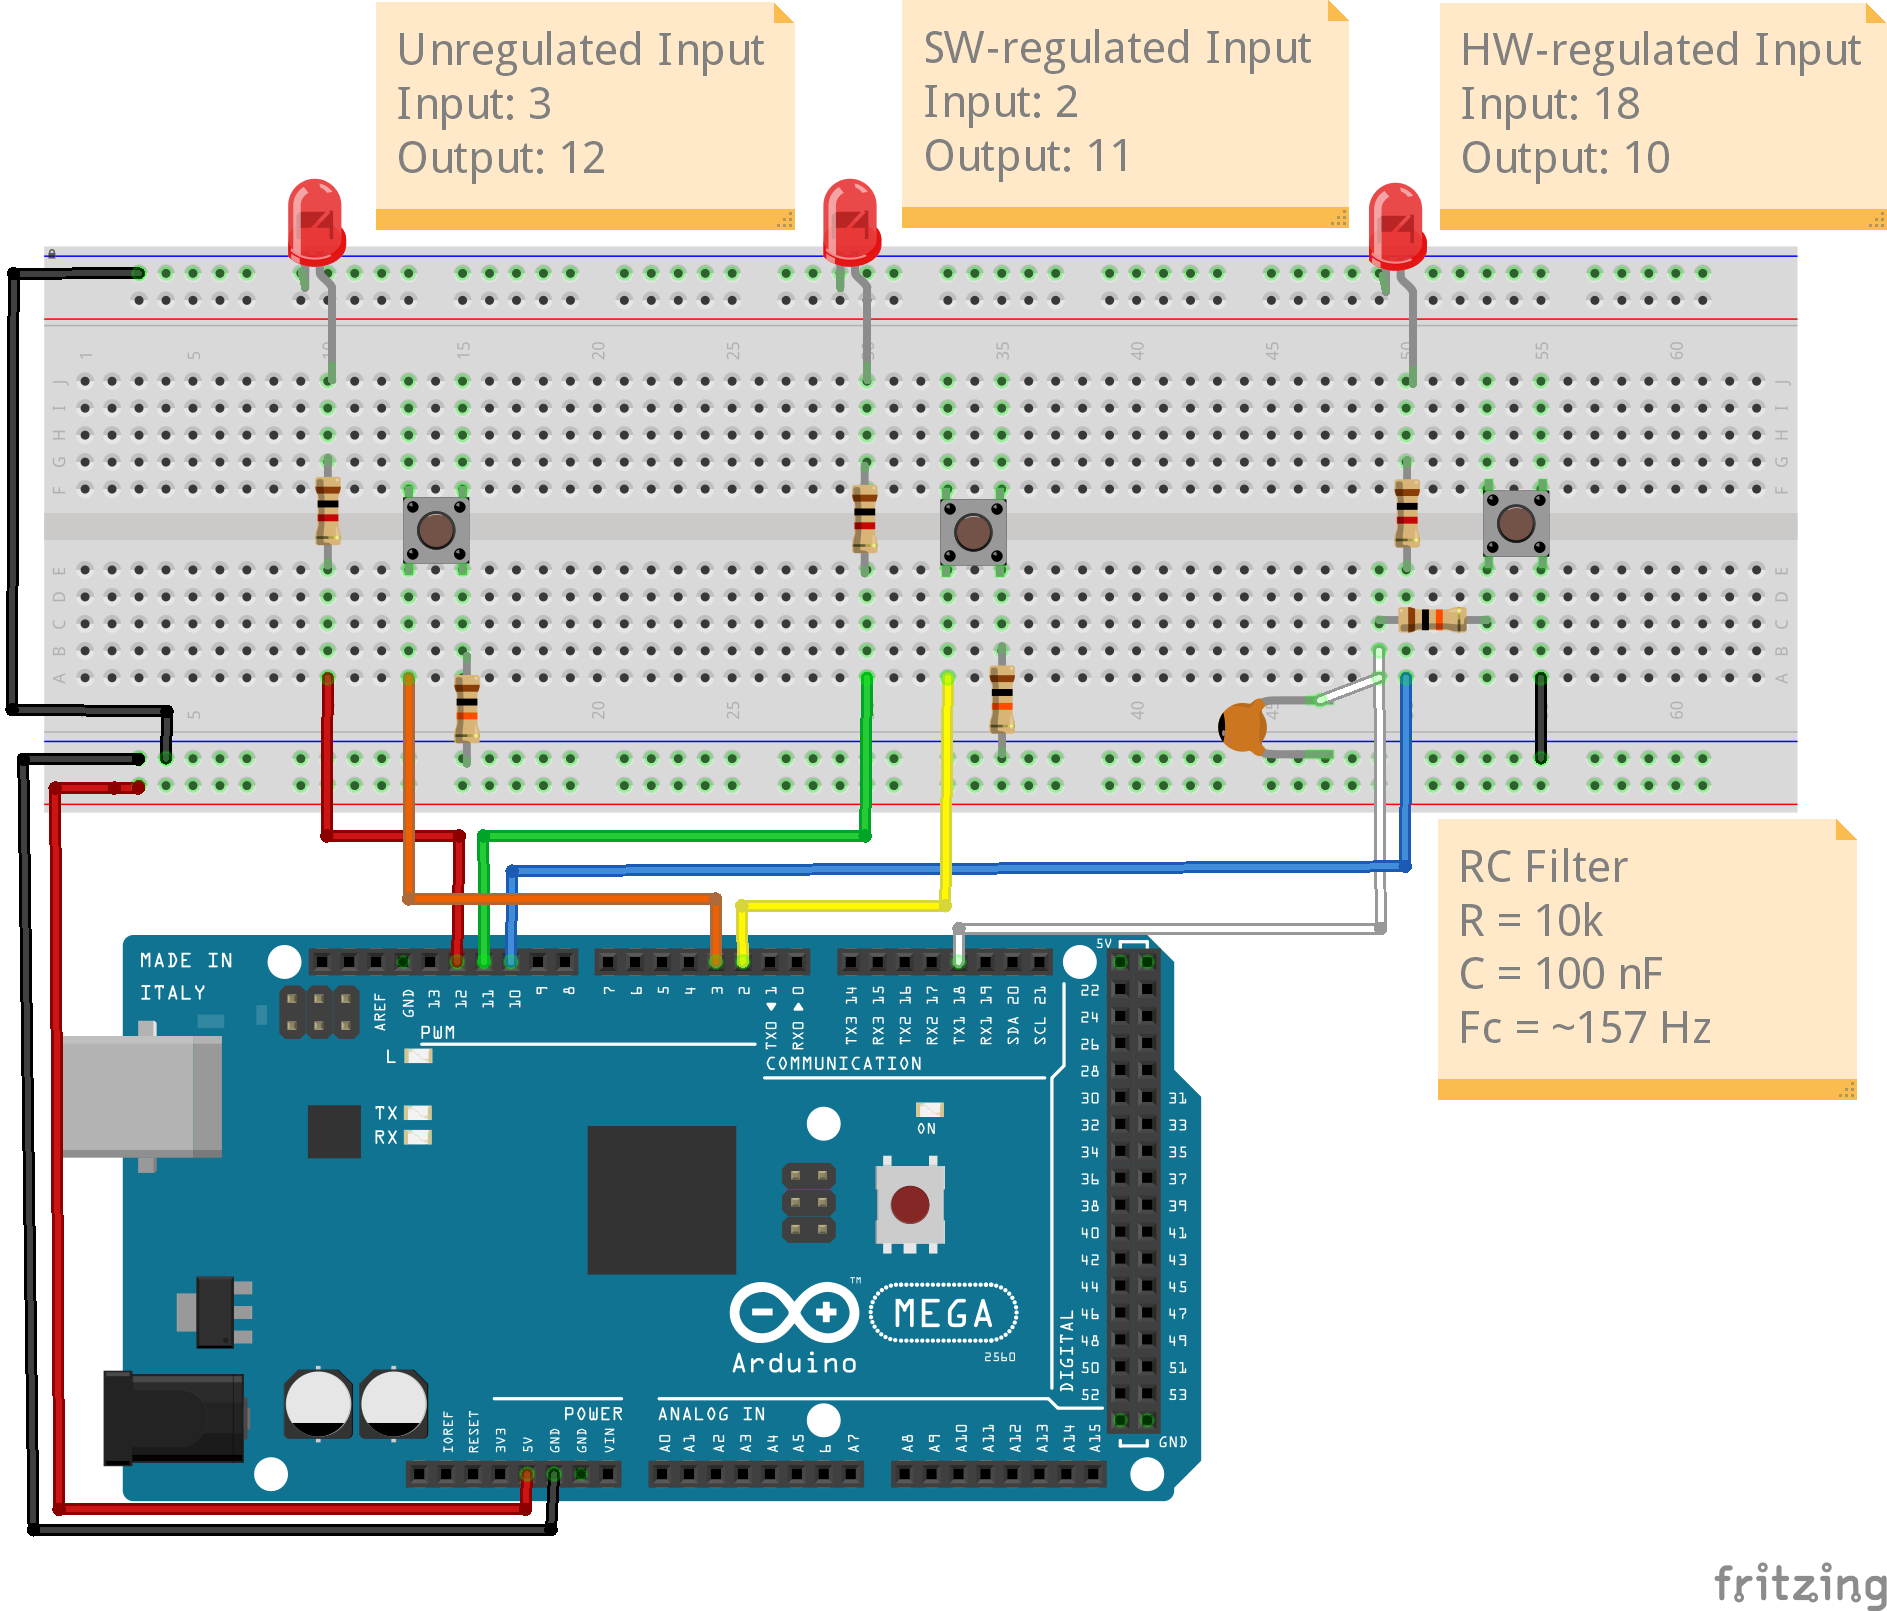
\includegraphics[]{p2_digital_inputs_bb.png}
        \caption{The breadboard layout for Project 2}
        \label{fig:p2_digital_inputs_bb}
    \end{figure*}

    \subsection*{Arduino Code}
    Students should have a well-organized and thought out program for this project.
    Firstly, they must declare and initialize the input and output pins being used as well as the counters for the number of button presses.
    Then, they must have created ISRs to perform the counter increments and printing for each button as well as change the LED state from on to off or vice versa.
    These interrupts must be attached to the appropriate input pins and, ideally, be triggered on the FALLING edge of the signal - though RISING could also work.
    The main loop of this function should just be setting the LED state for each LED since most of the logic will be handled asynchronously by the ISRs.

    For the sample code provided below, the pins are defined using the \lstinline[language=C++, style=mystyle]{#define} pre-compiler instruction and the LED states and counters are initialized.
    In \lstinline[language=C++, style=mystyle]{setup()} The Serial port is opened and the modes for the inputs and outputs are declared.
    Afterwards, the ISRs defined at the bottom of the code are attached to the input pins and set to trigger on the FALLING edge of the pin's signal (i.e. when the button is pressed and the voltage on the pin go towards 0).

    In \lstinline[language=C++, style=mystyle]{loop()}, the various LED states are written to the LED pins based on the global variable.
    The ISR code executes asynchronously, so nothing else is reuqired in this section

    Both \lstinline[language=C++, style=mystyle]{unregBtnISR()} and \lstinline[language=C++, style=mystyle]{hwregBtnISR()} do the same thing because the debouncing is either not handled or done so externally to the program.
    The software trick comes inside \lstinline[language=C++, style=mystyle]{swregBtnISR()}.
    Here, a static variable is initialized that will retain its value after the ISR is finished executing.
    This value holds the last known millisecond reading of the press detection logic.
    Then, the current millisecond reading is captured and used to compare with the previous value.
    If 100 ms have passed since the ISR was last executed, then the code block assumes it was a valid button press and increments the counter, changes the LED state, and prints out the counter to the Serial port.
    If an appropriate time has not passed, then the ISR assumes the detection was a bounce and resets the last millisecond reading before exiting.

    \pagebreak
    \lstinputlisting[language=C++, style=mystyle]{../../../src/projects/project_2_digital_inputs/project_2_digital_inputs.ino}
\end{document}